\documentclass[a4paper,11pt]{scrartcl}
\usepackage[french]{babel}
\usepackage[utf8]{inputenc}
\usepackage[T1]{fontenc}
\usepackage{pst-all}
\usepackage{vanadin}
\usepackage{isotope}
\usepackage{longtable}
\usepackage{color}
\usepackage{amsmath}
\usepackage{units}
\usepackage{float}


\subject{TP~3 Physique nucléaire}
\title{Perte d'énergie des particules $\alpha$ dans l'air}
\subtitle{Particules $\alpha$ dans l'air}
\author{Mona Dentler, Sabine Engelhardt}
\publishers{Université Joseph Fourier, Grenoble}
\date{\today}

\begin{document}
 \pagestyle{empty}
 \begin{center}
  \makeatletter
   %\titlefont
  \@subject
  \vspace{2cm}

  \Huge
  Perte d'énergie des particules $\alpha$ dans l'air\newline
  \vspace{1cm}
  \Large


  \@author
  \newline
  \@publishers


  \@date
  \makeatother
 \end{center}
 \vfill

 \begin{abstract}
  Le but des cette TP est de connaître la perte d'énergie des particules $\alpha$ dans l'air. Nous avons eu deux sources une source d'Americium 241 (\isotope[241]{Am}) et une source de Plomb 212/ Bismuth 212 (\isotope[212]{Bi}) pour étudier des particules $\alpha$ différentes. L'$\alpha$ perd son énergie par ionisation des atomes de la matière, ici l'air. La perte est proportionelle au carré de la charge et à la masse de l'$alpha$ et varie beaucoup avec la vitess d'$\alpha$. Plus l'$\alpha$ est lente plus de temps il passe dans l'atome et \c ca augmente la chance d'une interaction. Si l'ionisation est très intense, le trajet de la particule est très court.

  Dans ce TP nous allons étudier le spectre des $\alpha$ émis par les deux sources, calibrer le dispositif éxpermental pour ensuite mesurer le pouvoir d'ionisation des $\alpha$. C'est réalisé par la mesure de la longuer du trajet des $\alpha$ dans l'air.
 \end{abstract}
\newpage
 \pagestyle{scrheadings}
 \tableofcontents
\newpage

 \begin{section}{Etude des sources}
  \begin{subsection}{La source \isotope[241][95]{Am}}
   La période de l'\isotope[241][95]{Am} est \unit[432,6]{ans} et ce noyeau se désintègre vers le \isotope[237][93]{Np}. A presque \unit[100]{\%} des désintégration sont des désintégration $\alpha$, seule $\unit[4,3\cdot10^{-10}]{\%}$ 
   se fait par fission spontanée.\\
   \begin{figure}[H]
    \begin{center}
     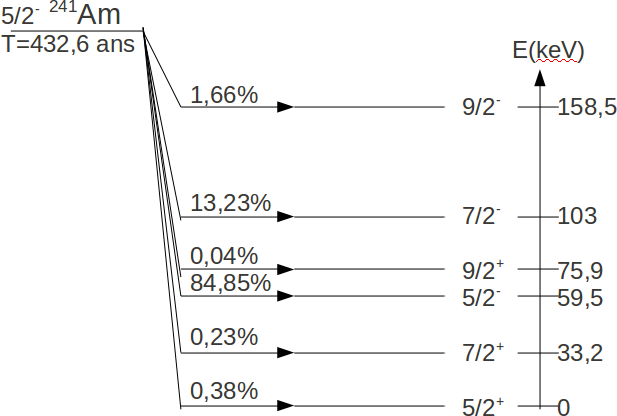
\includegraphics[width=0.5\textwidth]{Bilder/schemaAm1.png}
    \end{center}
    \caption{Schéma de désintégration de l'\isotope[241][95]{Am}}
   \end{figure}
   L'énergie libérée $Q$ par la désintégration est équivalent à la différence d'énergie causé par le défaut de masse entre les particules. Alors l'énergie cinétique $T$ des trois $\alpha$ principaux se calculent comme suivante:
   \begin{equation*}
    Q=\Delta E\stackrel{Einstein}{=}\Delta M\cdot c^2=\left[M\left(\isotope[241]{Am}\right)-M\left(\isotope[237]{Np}\right)-M\left(\isotope[4]{He}\right)\right]c^2\approx\unit[5,638]{MeV}
   \end{equation*}\\
   avec $M\left(\isotope[241]{Am}\right)=\unit[241,0568229]{uma},\text{ }M\left(\isotope[237]{Np}\right)=\unit[237,0481673]{uma}, \\ M\left(\isotope[4]{He}\right)=\unit[4,00266032]{uma}\text{ et }\unit[1]{uma}\cdot c^2=\unit[931,5]{MeV}$.\\
   L'énergie $Q^{\ast}$ des désintégrations vers les états excités s'y calcule par $Q^{\ast}=Q-E^{\ast}$.\\
   La conservation de la quantité de mouvement implique
   \begin{equation*}
    m(\alpha)T(\alpha)=m(Np)T(Np)
   \end{equation*}
   En outre la conservation de l'énergie totale a pour conséquence
   \begin{equation*}
    Q=T(Np)+T(\alpha)
   \end{equation*}
   On trouve donc pour l'énergie cinétique d'une particule $\alpha$ \isotope[4][2]{He}   
   \begin{equation*}
    T(\alpha)=\frac{m(Np)\cdot Q^{\ast}}{m(\alpha)+m(Np)}
   \end{equation*}
   Les trois $\alpha$ principaux sont ceux avec la plus grande possibilité d'être émis, ici ce sont les $\alpha$ émis par la désintégration vers \isotope[237]{Np^*} $\nicefrac{5}{2}^-$ avec \unit[84,85]{\%}, la désintégration vers \isotope[237]{Np^*} $\nicefrac{7}{2}^-$ avec \unit[13,23]{\%} et la désintégration vers \isotope[237]{Np^*} $\nicefrac{9}{2}^-$ avec \unit[1,66]{\%}. Alors on trouve pour leur énergie cinétique
   \begin{eqnarray*}
    T_{\nicefrac{5}{2}^-}=\unit[5,413]{MeV}\\
    T_{\nicefrac{7}{2}^-}=\unit[5,370]{MeV}\\
    T_{\nicefrac{9}{2}^-}=\unit[5,316]{MeV}
   \end{eqnarray*}
  \end{subsection}
 
  \begin{subsection}{La source \isotope[212][83]{Bi}}
   Le \isotope[212][83]{Bi} fait partie de la chaîne radioactive du Thorium 232. Car le  \isotope[212]{Bi} n'a qu'une période de \unit[60,5]{min}, la source a été apporté par un technicien pendant la TP. Le \isotope[212]{Bi} se désintègre vers le Thalium \isotope[208][81]{Tl} en émettant des particules $\alpha$ \isotope[4][2]{He} et vers le Polonium\isotope[212][84]{Po} par désintégration $\beta^-$ comme le schéma suivant le montre.\\
   \begin{figure}[H]
    \begin{center}
     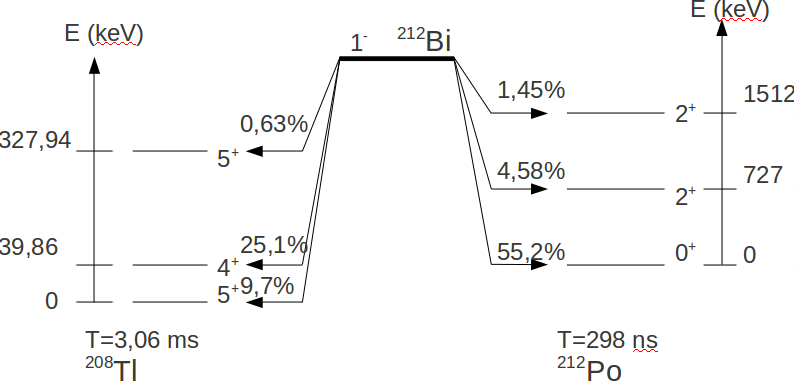
\includegraphics[width=0.75\textwidth]{Bilder/schemaBi1.png}
    \end{center}
    \caption{Schéma de désintégration du \isotope[212][83]{Bi} }
   \end{figure}
   On peut se poser la question pourquoi la désintégration du \isotope[212]{Bi} vers l'état fondamental est plus probable que vers le deuxième état excité parce qu'ils ont tous les deux le même moment angulaire et la même parité $5^+$. C'est assez facile à comprendre car les atomes vont avoir un état énergétiquement favorable, c'est à dire un état stable. Comme l'état fondamental est le plus stable des deux états la désintégration vers l'état fondamental est préféré.\\
\newpage
   Le Polonium \isotope[212][84]{Po} fait à son tour par \unit[100]{\%} la désintégration $\alpha$ vers le plomb \isotope[208][82]{Pb} avec une période de $T=\unit[298]{ns}$. Cette période est très couret à cause de la préférence d'un noyeau avec un nombre magique. Le \isotope[208][82]{Pb} est un noyeau double magique avec le nombre magique 84 pour les protons et le nombre magique 126 pour les neutrons. Alors ce noyeau est fortement favorisé du noyeau de \isotope[212]{Po}.
   \begin{figure}[H]
    \begin{center}
     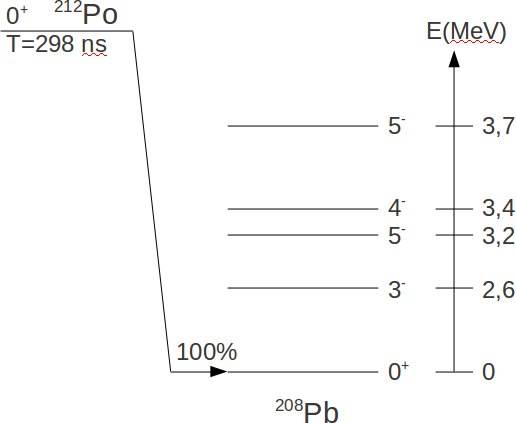
\includegraphics[width=0.5\textwidth]{Bilder/schemaPo1.png}
    \end{center}
    \caption{Schéma de désintégration du \isotope[212][84]{Po} }
   \end{figure}
   Les trois $\alpha$ principaux de la désintégration du \isotope[212]{Bi} sont deux $\alpha$ de la désintégration vers le \isotope[208]{Tl} et l'$\alpha$ de la désintégration du \isotope[212]{Po}. Pour 100 désintégration du \isotope[212]{Bi} environ 90 particules $\alpha$ sont émis et nous avons calculé l'énergie cinétique des trois $\alpha$ principaux.
   \begin{eqnarray*}
    Q_{5^+}(Bi)&=\left[M\left(\isotope[212]{Bi}\right)-M\left(\isotope[208]{Pb}\right)-M\left(\isotope[4]{He}\right)\right]c^2\approx\unit[6,154]{MeV} &\text{ avec }\unit[9,7]{\%}\\
    &\rightarrow T_{0}(\alpha)=\unit[6,042]{MeV}\\
    Q_{4^+}(Bi)&=Q_0-E^*_{4^+}=\unit[6,114]{MeV} &\text{ avec }\unit[25,1]{\%}\\
    &\rightarrow T_{2^+}(\alpha)=\unit[6,004]{MeV}\\
    Q_{0^+}(Po)&=\left[M\left(\isotope[212]{Po}\right)-M\left(\isotope[208]{Pb}\right)-M\left(\isotope[4]{He}\right)\right]c^2\approx\unit[8,954]{MeV} &\text{ avec }\unit[55,2]{\%} \\  
    &\rightarrow T_{0}(\alpha)=\unit[8,785]{MeV}\\
   \end{eqnarray*}
   avec $M\left(\isotope[212]{Bi}\right)=\unit[211,9912715]{uma},\text{ }M\left(\isotope[208]{Tl}\right)=\unit[207,9820047]{uma}, M\left(\isotope[212]{Po}\right)=\unit[211,9888518]{uma},\newline M\left(\isotope[208]{Pb}\right)=\unit[207,9766359]{uma}, M\left(\isotope[4]{He}\right)=\unit[4,00266032]{uma}\text{ et }\unit[1]{uma}\cdot c^2=\unit[931,5]{MeV}$.
  \end{subsection}
 \end{section}
\newpage
 \begin{section}{Dispositif expérimental}
  Le dispositif expérimental se compose d'un enceinte à vide et ses accesoires, un détecteur rélie à un préimplificateur et un analyseur multicanal. Le siganl est enregisté sur l'ordinateur par un logiciel très simple.
  \begin{subsection}{Enceinte à vide}
   Dans l'einceinte à vide se trouve le détecteur et un sélecteur de source pour que nous n'ayons pas dû toucher les sources nues $\alpha$ se qui est très dangereux et peut causé de cancer. En plus il y a une pompe pour faire le vide et un système de vanne et de fuit micrométrique pour faire rentrer l'air précisement. Un jauge capacitif calibré parun jauge Pirani très précis mesure la pression dans l'enceinte avec une précision de \unit[0,2]{\%}.  
  \end{subsection}

  \begin{subsection}{Détecteur et préamplificateur}
\enlargethispage{1cm}
   \begin{figure*}[hbt]
    \begin{center}
     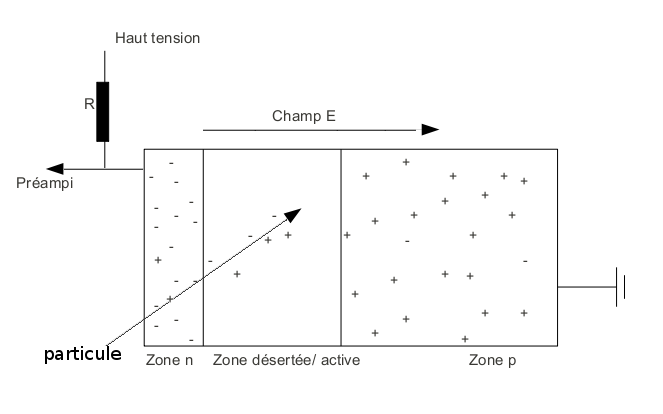
\includegraphics[width=0.75\textwidth]{Bilder/detecteur.png}
    \end{center}
    \caption{Schéma d'un détecteur semi-conducteur}
   \end{figure*}
   Le détecteur est un détecteur semi-conducteur et consiste d'une jonction Si(Li) avec une barrière de surface. Un détecteur semi-conducteur a trois parts: une zone chargée négative n, une zone chargée positive p  et une zone neutre, la zone active ou desertée. Le largeur de cette dernière zone est reglée par haute tension, la tension de polarisation. Comme ci la jonction est assimilable à un condensateur plan dont la distance est égale à la zone désertée. Donc ce condensateur est de même d'amplitude que la tension rélié.
   Le préamplificateur de charge supprime ce problème. Il est rélie à un module de mise en forme qui fournit un signal de l'amplitude proportionel à la charge collecté dans la jonction du détecteur indépedant de la capacité.
  \end{subsection}

  \begin{subsection}{Logiciel}
   Un amplificateur entre le préamplificateur et l'analyseur d'amplitude donne la possibilité d'ajuster le signal à un valeur connue. L'analyseur d'amplitude est rélie à l'ordinateur où un logiciel montre le signal en fonction de l'énergie d'$\alpha$. Ce logiciel n'est pas calibré alors il faut le faire soi-même et il permet de choisir la temps de la mesure et un seuil qui était mis à \unit[200]{mV}.
  \end{subsection}
 \end{section}
  
 \begin{section}{Expériences préliminaire}
  \begin{subsection}{Etude de la réponse du détecteur}
   \begin{subsubsection}{Caractéristique du détecteur}
   Nous avons utilisé le logiciel \flqq Astar \frqq \. pour avoir une estimation de l'énergie maximale pour laquelle la particule perd toute son énergie.  Les énergies utilisés pour les calculations du Total Stopping Power et du Projected Range étaient les plus probables des désintégration. La première mesure était fait pour le détecteur donc le matériel donné est Silicium, la deuxième mesure était fait pour l'air.
   \begin{paragraph}{Silicium}
    \begin{center}
     \begin{tabular}{c|c|c|c}
      Désintegration&	Energie cinétique [MeV] & Total Stp. Pow. [$\frac{MeV cm^2}{g}$]  & Projected Range [$\frac{g}{cm^2}$] \\ \hline
      Am 	&5,413 & 584,6 & 0,00625 \\ 
      Bi	&6,004 & 546,7 & 0,00792 \\ 
      Po	&8,785 & 411,1 & 0,01313 \\ 
     \end{tabular}
    \end{center}
    Pour le détecteur on a donné und valeur de $\unit[1,5]{cm^2}$, donc les énergies maximale se calcule comme suivante 
    \begin{eqnarray*}
     E_{max}(Am)&=\text{Total Stp. Power}\cdot \unit[1,5]{cm^2}&=\unit[876,9]{MeV}\\
     E_{max}(Bi)&&=\unit[820,05]{MeV}\\
     E_{max}(Po)&&=\unit[616,65]{MeV}
    \end{eqnarray*}
    La densité du Silicium est $\rho=\unit[2,336]{\frac{g}{cm3}}$, alors on trouve pour les trajets maximale dans le détecteur
    \begin{eqnarray*}
     x_{max}(Am)&=\frac{\text{Projected Range}}{\rho}&=\unit[26,76]{\mu m}\\
     x_{max}(Bi)&&=\unit[33,92]{\mu m}\\
     x_{max}(Po)&&=\unit[56,21]{\mu m}
    \end{eqnarray*}
    \todo{rausfinden Spannung...}
   \end{paragraph}
   \begin{paragraph}{Air}
    \begin{center}
     \begin{tabular}{c|c|c|c}
      Désintégration & Energie cinétique \unit{[MeV]} & Total Stp. Pow. [$\frac{MeV cm^2}{g}$] & Projected Range [$\frac{g}{cm^2}$] \\ \hline
      Am & 5,413 & 718,0 & 0,00491 \\ 
      Bi & 6,004 & 669,3 & 0,00574 \\ 
      Po & 8,785 & 509,5 & 0,01055 \\ 
     \end{tabular}
    \end{center}
    Pour l'air seulement les trajets maximale sont intéressant et la densité de l'air dans l'atmosphère ambiante est $\rho\approx\unit[0,00129]{\frac{g}{cm^3}}$
    \begin{eqnarray*}
     x_{max}(Am)&=\frac{\text{Projected Range}}{\rho}&=\unit[38,06]{mm}\\
     x_{max}(Bi)&&=\unit[44,50]{mm}\\
     x_{max}(Po)&&=\unit[81,78]{mm}
    \end{eqnarray*}
    Nous avons que la distance maximale entre la source et le détecteur est \unit[45]{mm}, donc nous avons seulement la chance de détecter les pic de Bragg de la désintégration du Am et du Bi vers Tl.
   \end{paragraph}

     
   \end{subsubsection}

   \begin{subsubsection}{Largeur de la zone active en fonction de la tension}
    Pour comprendre le comportement du détecteur en fonction de la tension, nous avons lancé une série de mesure. Nous avons choisi une tension de \unit[0]{V}, \unit[25]{V}, \unit[50]{V} et \unit[80]{V} et nous avons mesurer à une pression de \unit[0,78]{mbar} pendant \unit[30]{s} par mesure.\\
    Nous avons aussi calculé la résolution en énergie $\frac{\Delta E}{E}$ en usant le savoir que la position du pic est proportionel à l'énergie.
    \begin{paragraph}{Résultat} 
     \begin{center}
      \begin{tabular}{c|c|c|c|}
       tension\unit{[V]} & $n^{\circ}$ de particules & Position	& Largeur du pic 	\\ \hline 
       0	&	2545,3  $\pm$ 50,45	&	1295,22	$\pm$ 3,21	&	14,36 $\pm$ 0,26		\\ 
       25	&	2154,9 $\pm$ 46,42	&	1664,71	$\pm$ 0,27	&	6,34 $\pm$ 0,18		\\ 
       50	&	1838,12 $\pm$ 42,87	&	1676,8	$\pm$ 0,28	&	4,93 $\pm$ 0,18		\\ 
       80	&	2028,32 $\pm$ 45,04	&	1678,01	$\pm$ 0,21	&	4,94 $\pm$ 0,14		\\ 
      \end{tabular}
     \end{center}
     L'intégrale du pic correspond à la nombre des particules mesurées et sa largeur à l'écart-type de la position.
 
     On voit bien qu'on a la plus petite erreur des  énergies avec la tension de \unit[80]{V}. C'est celui que nous avons utilisé pour tous les mesures suivantes. 
    \end{paragraph}

    \begin{paragraph}{Explication}
     On a vu qu'il est nécessaire que l'énergie des $\alpha$ est totalement perdue dans la zone desertée pour avoir un résultat exact. La zone agraindi proportionellement à la tension de polarisation.
    \end{paragraph}
   \end{subsubsection}
  \end{subsection} 

  \begin{subsection}{Calibration des résultat}
   Le logiciel \flqq Spectro TP\frqq ne donne que la position des pics, mais on ne sait pas à quoi \c ca correspond, alors il faut le calibrer. Ainsi nous avons fait une mesure pour chaque source avec une tension de \unit[80]{V} et une pression de \unit[0,78]{mb} en comptant pendant \unit[300]{s} pour avoir une mesure précise. Donc la pression est très petite on peut admettre que le trajet est zéro et en résulte que l'énergie des $\alpha$ donné au détecteur correspond à leur énergie maximale.
   \begin{paragraph}{Résultat}
    \begin{center}
     \begin{tabular}{c|c|c|c|c}
      Pic	& Energie [MeV] &	Position	&	Résolution	&	Nb de particules	\\ \hline
      Bi(Tl)	&6, 114	 &1868,94 $\pm$ 0,25 	&8,36 $\pm$ 0,25	&1215,24 $\pm$ 34,86	\\
      Bi(Po)	&8, 785	&2752,96 $\pm$ 0,12	&4,58 $\pm$ 0,08	&2335,28 $\pm$ 48,32	\\ 
      Am	&5, 433 &1662,27 $\pm$ 0,1	&13,52 $\pm$ 0,06	&23528,39 $\pm$ 153,39	\\ 
     \end{tabular}
    \end{center}
    \begin{figure}[H]
     \begin{center}
      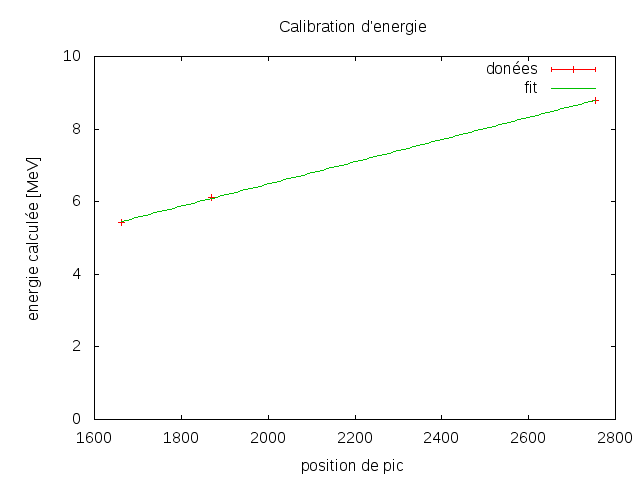
\includegraphics[width=0.75\textwidth]{Bilder/calibration.png}
      \caption[calibration d'énergie]{fitparameter: $ a = 0.00305786  \pm 4.301\cdot 10^{-5} \hspace{2 em} b = 0.371954  \pm 0.09235$ }
     \end{center}
    \end{figure}
   \end{paragraph}
   Nous savons l'énergie des $\alpha$ et la position de pic, en faisant la supposition que l'augmentation de la position de pic est linéair à l'augmentation de l'énergie nous avon fait un fit en utillisant le logiciel \flqq Gnuplot\frqq\. qui applique la méthode des moindres carrés. On trouve pour les coefficients a et b les valeurs
   \begin{align*}
    a&= 0.00305786 \\
    b&= 0.371954 \\
    \rightarrow E_{callibration} &= 0.00305786  \cdot E +0.371954 
   \end{align*}
  \end{subsection}

  \begin{subsection}{Simulation de la perte d'énergie}
   Nous avons lancé une simulation avec le logiciel \flqq SRIM \frqq pour savoir quoi attendre. Nous avons pris pour la simulation un trajet de \unit[45]{mm} (la distance maximale entre la source et le détecteur) dans l'air.
   \begin{figure}[H]
    \begin{minipage}{0.45\textwidth}
     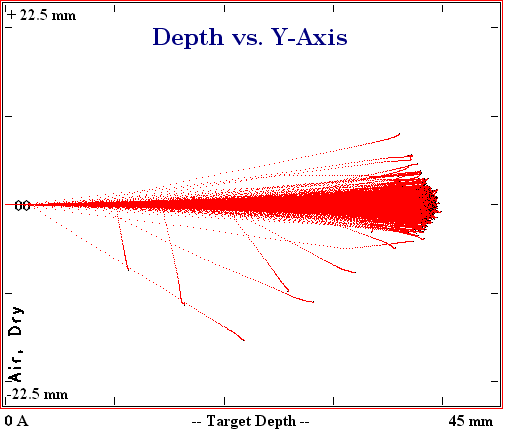
\includegraphics[width=\textwidth]{Bilder/simam.png}
     \caption{Simulation avec une énergie de \unit[5]{MeV} pour l'\isotope[241]{Am}}
    \end{minipage}
    \hfill
    \begin{minipage}{0.45\textwidth}
     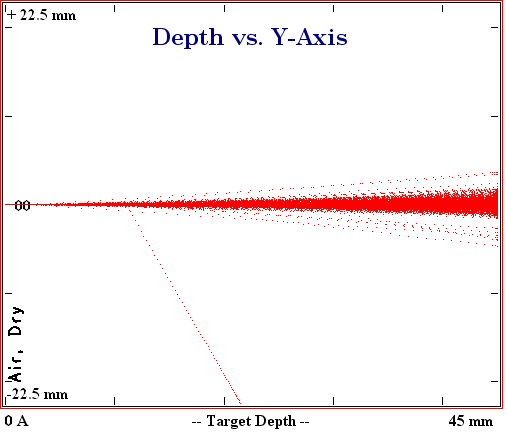
\includegraphics[width=\textwidth]{Bilder/simbi7MeV.png}
     \caption{Simulation avec une énergie de \unit[7]{MeV} pour le \isotope[212]{Bi}}
    \end{minipage}
   \end{figure}
   On va bien que les particules $\alpha$ de l'\isotope[241]{Am} n'arrivent pas au détecteur au contraire aux particules $\alpha$ du \isotope[212]{Bi}. Cela veut dire pour nous qu'il faut absolument mesure l'\isotope[241]{Am} car là nous trouverons bien les pic de Bragg. Pour le \isotope[212]{Bi} il fallait mesurer encore des trajets plus longs qui n'étaient pas possible avec notre dispositif éxperimental. Car nous avons pris à peu près le moyenne des énergies possible pour le \isotope[212]{Bi} c'est possible de trouver le pic de Bragg pour les désintégrations vers le \isotope[208]{Tl} avec une énergie d'environ \unit[6]{MeV}.
  \end{subsection}
 \end{section}

 \begin{section}{Mesure de l'atténuation des particules alpha dans l'air}
  \begin{subsection}{Perte d'énergie dans l'air en fonction de pression}
   \begin{subsubsection}{La source \isotope[241][95]{Am}}
    \begin{center}
     \begin{tabular}{c|c|c|c|c|c|c|c}
      pression\unit{[mb]} & $n^{\circ}$ du pic	&	énergie	&	err(én)	&	Largeur du pic	&	err(res)	&	$n^{\circ}$ de particules	&	err(part) 	\\ \hline
      1,62	&	1	&	1660,02	&	0,25	&	6,83	&	0,21	&	1486,168	&	38,55	\\ 
      102,4	&	1	&	1525,79	&	0,29	&	8,7	&	0,25	&	1542,36	&	39,27	\\ 
      199,7	&	1	&	1374,82	&	0,33	&	10,99	&	0,26	&	1600,78	&	40,01	\\ 
      300,5	&	1	&	1216,61	&	0,4	&	13,96	&	0,32	&	1674,84	&	40,92	\\ 
      401,3	&	1	&	1044,07	&	0,52	&	18,31	&	0,45	&	1664,61	&	40,8	\\ 
      501,08	&	1	&	855,9	&	0,59	&	21,59	&	0,49	&	1695,65	&	40,74	\\ 
      608,7	&	1	&	609,86	&	0,72	&	26,56	&	0,6	&	1615,09	&	40,19	\\ 
      706,3	&	1	&	349,35	&	1,17	&	30,9	&	1,31	&	1341,7	&	36,63	\\ 
      706,3	&	2	&	246,13	&	36,48	&	128,45	&	32,14	&	474,96	&	21,31	\\ 
      806,39	&	1	&	246,13	&	36,48	&	128,45	&	32,14	&	474,96	&	21,31	\\ 
      653,9	&	1	&	503,98	&	0,86	&	29,08	&	0,77	&	1511,56	&	38,8	\\ 
      714,65	&	1	&	329,75	&	1,16	&	32,07	&	1,26	&	1402,57	&	37,45	\\ 
      714,65	&	2	&	207,4	&	42,1	&	116,78	&	35,28	&	362,95	&	19,05	\\ 
      738,8	&	1	&	247,17	&	1	&	40,16	&	1,2	&	1525,44	&	39,05	\\ 
      762,2	&	1	&	172,24	&	1,36	&	45,47	&	1,32	&	1475,01	&	38,41	\\ 
      774,5	&	1	&	134,43	&	1,3	&	40,26	&	1,26	&	1290,85	&	35,93	\\ 
      817,3	&	1	&	134,43	&	1,3	&	40,26	&	1,62	&	1290,9	&	35,92	\\ 
		&	-	&		&		&		&		&	14	&		\\ \hline
      \hline
      \multicolumn{ 6}{|c|}{} & temps\unit{[s]} & 20 \\ \cline{ 7- 8}
      \multicolumn{6}{|c|}{} & tension \unit{[V]}& 80 \\ \cline{7-8}
      \multicolumn{ 6}{|c|}{} & matériau& \isotope[241][95]{Am} \\ \hline
     \end{tabular}
    \end{center}
   \end{subsubsection}

   \begin{subsubsection}{La source \isotope[212][83]{Bi}}
    
   \end{subsubsection}
  
   \begin{subsubsection}{La source \isotope[212][82]{Po}}
    
   \end{subsubsection}


    
   \begin{table}[H]
    \caption{Energie des alphas en fonction de pression pour le \isotope[212][83]{Bi}}
    \begin{center}
     \begin{tabular}{c|c|c|c|c|c|c|c}

      pression\unit{[mb]} & pic	&	énergie	&	err(én)	&	Largeur du pic	&	err(res)	&	$n^{\circ}$ de particules	&	err(part) 	\\ \hline
      6,43	&	1	&	2732,85	&	0,23	&	5,69	&	0,26	&	412,9	&	20,32	\\ 
      6,43	&	2	&	1899,94	&	0,63	&	9,11	&	0,65	&	242,96	&	15,59	\\ 
      100,7	&	1	&	2653,17	&	0,36	&	7,28	&	0,33	&	460,25	&	21,5	\\ 
      100,7	&	2	&	1741,73	&	0,85	&	11,2	&	1,06	&	253,24	&	25,11	\\ 
      200,42	&	1	&	2564,43	&	0,45	&	8,97	&	0,42	&	445,97	&	21,12	\\ 
      200,42	&	2	&	1619,05	&	1,4	&	14,61	&	2,21	&	177,23	&	13,21	\\ 
      300,6	&	1	&	2461,22	&	0,6	&	11,52	&	0,62	&	429,58	&	20,73	\\ 
      300,6	&	2	&	1474,6	&	1,61	&	18,89	&	1,98	&	235,1	&	15,33	\\ 
      403,7	&	1	&	2357,18	&	0,73	&	12,27	&	0,7	&	379,64	&	19,48	\\ 
      403,7	&	2	&	1326,71	&	1,59	&	18,99	&	2,33	&	226,68	&	15,06	\\ 
      503,7	&	1	&	2246,3	&	0,85	&	15,47	&	0,83	&	413,87	&	20,34	\\ 
      503,7	&	2	&	1161,31	&	2,08	&	24,58	&	2,86	&	234,92	&	15,32	\\ 
      605,2	&	1	&	2143,09	&	0,95	&	16,41	&	1,01	&	387,72	&	19,69	\\ 
      605,2	&	2	&	1001,36	&	4,3	&	39,75	&	9,3	&	297,97	&	17,26	\\ 
      705	&	1	&	2029,47	&	1,17	&	15,54	&	1,17	&	309,43	&	17,59	\\ 
      705	&	2	&	1152,52	&	116,51	&	70,93	&	202,05	&	3526,06	&	59,38	\\ 
      802,1	&	1	&	1916,84	&	1,08	&	19,65	&	1,37	&	387,17	&	19,68	\\ 
      802,1	&	2	&	626,78	&	71,36	&	253,05	&	113,1	&	987,4	&	31,42	\\ 
      905,2	&	1	&	1793,34	&	1,42	&	16,75	&	1,89	&	257,1	&	16,03	\\ 
      994,66	&	1	&	1678,34	&	1,64	&	27,11	&	2,01	&	401,01	&	29,03	\\ \hline
      \hline
      \multicolumn{ 6}{|c|}{} & temps\unit{[s]} & 30 \\ \cline{ 7- 8}
      \multicolumn{6}{|c|}{} & tension \unit{[V]}& 80 \\ \cline{7-8}
      \multicolumn{ 6}{|c|}{} & matériau& \isotope[212][83]{Bi} \\ \hline
     \end{tabular}
    \end{center}
   \end{table}
   \begin{figure*}[H]
    \begin{center}
     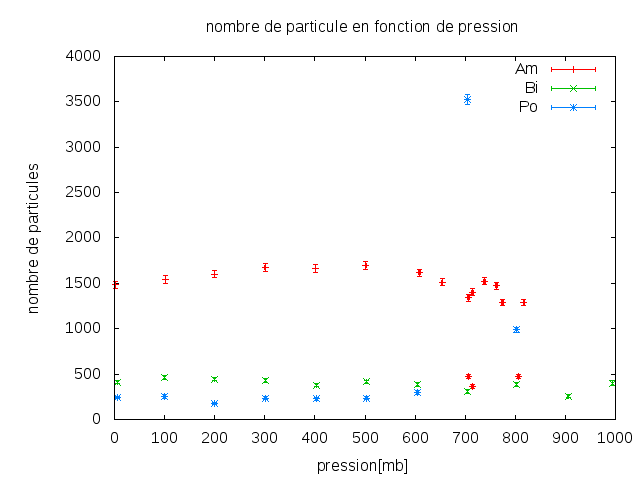
\includegraphics[width=0.75\textwidth]{Bilder/fonction_pression.png}
    \end{center}
   \end{figure*}
   Le dispositif expérimental est construit ainsi que la distance entre le détecteur et la source est fixé à \unit[45]{mm}. Donc on modifie la pression d'air à l'intérieur de l'enceinte à vide pour simuler des distances différentes.\\
   L'équation des gaz parfaits $p \cdot x \cdot A =N \cdot R \cdot T$ nous indique que la pression $p$ et la distance $x$ sont inversement proportionelles, il en résulte pour la distance x = x(p) 
   \begin{equation*}
    x=\frac{p}{p_0}\cdot x_0
   \end{equation*}
\newpage
   Avec la calibration d'énergie $E_{callibration}= 0.00305786  \cdot E +0.371954 $, on trouve pour le distance $x$ en fonction d'énergie $E$:
   \begin{figure*}[h]
    \begin{center}
     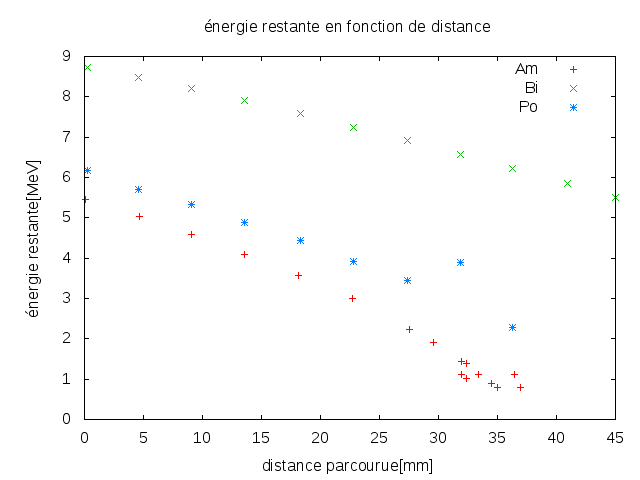
\includegraphics[width=0.75\textwidth]{Bilder/energie_restante.png}
    \end{center}
   \end{figure*}
   \begin{figure*}[h]
    \begin{center}
     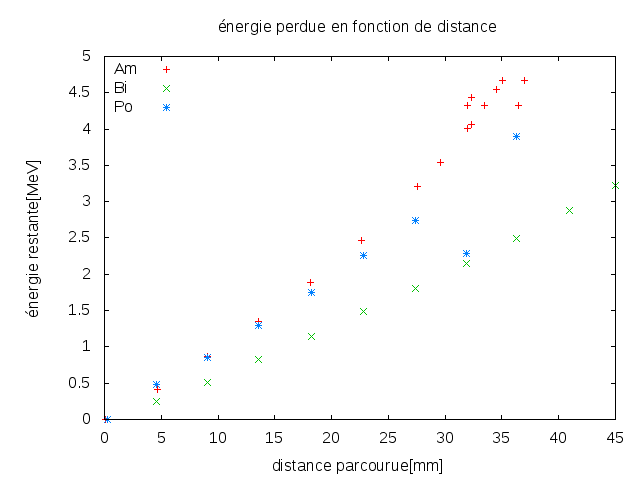
\includegraphics[width=0.75\textwidth]{Bilder/energie_perdue.png}
    \end{center}
   \end{figure*}
  \end{subsection}
  
  \begin{subsection}{Perte d'énergie par unité de longueur}
  \end{subsection}
 \end{section}

 \begin{section}{Pic de Bragg}
  
 \end{section}

 
 \begin{section}{Conclusion}
  Nous avons appris comment lancé une mesure et calibré les dispositifs pour cette mésure. En plus nous avons vu que des particules $\alpha$ déposent leur énergie après un certain trajet parcouru. Cette distance montré par le pic de Bragg est spécifique pour les $\alpha$ d'une source comme nous avons vu en comparaisant les deux sources disponibles pour la TP.
  
  Dans la radiothérapie on use ce fait pour détruire des tumeurs. En utilisant des particules $\alpha$ on est sûre de ne détruire que la tumeur car l'alpha interagissent que dans cette pétite zone bien défini.
 \end{section}

 \vspace{1cm}
 \begin{flushright}
  \titlefont \textcopyleft\ Mona Dentler et Sabine Engelhardt
 \end{flushright}

\end{document}

